\documentclass[12pt]{article}
\usepackage{lingmacros}
\usepackage{tree-dvips}
\usepackage{amsmath}
\usepackage{IEEEtrantools}
\usepackage{amssymb}
\usepackage{graphicx}
\usepackage{float}
\usepackage{sectsty}
\usepackage{xstring}
\usepackage{xparse}

\usepackage{mleftright}
\mleftright

\usepackage{amsthm}
\newtheorem{theorem}{Theorem}

\usepackage{cancel}

\interdisplaylinepenalty=100
% \interdisplaylinepenalty=10
% \interdisplaylinepenalty=0

\usepackage[colorlinks=true,linkcolor=blue]{hyperref}
\makeatletter
\def\IEEElabelanchoreqn#1{\bgroup
\def\@currentlabel{\p@equation\theequation}\relax
\def\@currentHref{\@IEEEtheHrefequation}\label{#1}\relax
\Hy@raisedlink{\hyper@anchorstart{\@currentHref}}\relax
\Hy@raisedlink{\hyper@anchorend}\egroup}
\makeatother
\newcommand{\subnumberinglabel}[1]{\IEEEyesnumber
\IEEEyessubnumber*\IEEElabelanchoreqn{#1}}

\usepackage[dvipsnames]{xcolor}

\graphicspath{ {./images/} }
\iffalse
	\sectionfont{\fontsize{16}{15}\selectfont}
\fi

% *** Magic Commands! *** %

	% call empty: \coherent[]{S}
	% call with index: \coherent[0]{S+l}
	\NewDocumentCommand\coherent{om}{%
		\IfNoValueTF{#1}
		{$|#2\rangle$}
		{$|#2_#1\rangle$}%
	}

	\newcommand{\logH}[1]{#1\log{\left[\frac{1}{#1}\right]}}
	\newcommand{\logHminus}[1]{#1\log{#1}}

	\newcommand{\lambdaWave}{\overline{\lambda}}
	\newcommand{\curlyBracket}[1]{
		\begin{equation*}
			\left\{ \,
			\begin{IEEEeqnarraybox}[][c]{l"s}
				\IEEEstrut
					#1
				\IEEEstrut
			\end{IEEEeqnarraybox}
			\right.
		\end{equation*}
	}
	\newcommand{\curlyBracketFull}[2]{
		\begin{equation*}
			#1 \left\{ \,
			\begin{IEEEeqnarraybox}[][c]{l"s}
				\IEEEstrut
					#2
				\IEEEstrut
			\end{IEEEeqnarraybox}
			\right.
		\end{equation*}
	}
	\newcommand{\lambdaSwitch}[1]{%
		\IfEqCase{#1}{%
			{0}{\lambda_0=|S_0+l|^2}%
			{1}{\lambda_1=|S_1+l|^2}%
			{i}{\lambda_i=|S_i+l|^2}%
			{~}{\widetilde{\lambda}=\pi_{0}\sqrt{\lambda_{0}}+\pi_{1}\sqrt{\lambda_{1}}}%
			{-}{\lambdaWave=\pi_{0}\lambda_{0}+\pi_{1}\lambda_{1}}%
		}[\PackageError{tree}{Undefined option to tree: #1}{}]%
	}%

	
	\newcommand{\g}{g = \frac{\pi_{0}}{\pi_{1}}}
	\newcommand{\lStar}{\frac{S_{0}\pi_{0} - S_{1}\pi_{1}}{\pi_{1}-\pi_{0}}}
	
	\newcommand{\piG}[1]{%
		\IfEqCase{#1}{%
			{0}{\frac{g}{1+g}}%
			{1}{\frac{1}{1+g}}%
		}[\PackageError{tree}{Undefined option to tree: #1}{}]%
	}%

% *********************** %

	\def\changemargin#1#2{\list{}{\rightmargin#2\leftmargin#1}\item[]}
	\let\endchangemargin=\endlist 

% *********************** %

\begin{document}

	\begin{center}
		\section*{Signal detection over an optical channel}
	\end{center}

	\vspace{0.3cm}

	Given an optical channel, a signal on that channel can be described as a coherent state denoted by \coherent{S} where  $S\in\mathbb{C}$
.\\\par
	Considering a Noise free environment, in order to detect a signal in this type of channel, 
	we use a photon counter receiver. Such a receiver is a direct detection receiver which detects 
	the intensity of the optical and generates a Poisson process, where the rate of the process holds $\lambda = |S|^2$ 
.\\\par
	Suppose we have two coherent state signals denoted by \coherent[0]{S}, \coherent[1]{S} and we would like to distinguish between the two 
	binary hypotheses with the corresponding priori probabilities $\pi_0, \pi_1$ respectively under hypotheses $H=0,1$, 
	while holding some transmission cost constraint
.\\\par
	One approach was given by \textbf{Kennedy} who proposed adding a constant additional coherent state signal \coherent{l}
	before feeding the signal’s input to the receiver. Doing so generates a coherent state \coherent{S+l} which 
	the receiver in turn outputs a Poisson process with rate $\lambdaSwitch{i}$
.\\\par
	An additional approach was given by \textbf{Dolinar} who suggested as continuation to Kennedy’s design to replace the constant 
	signal with a controlled signal \coherent{l(t)} which is chosen adaptively based on the photon arrivals up to that moment, 
	in order to achieve more certainty in the hypothesis choice with time
.\\\par
	The core concept of Dolinar’s updated design includes a recursive method in which the posterior probabilities of 
	the two possible hypotheses denoted by $\pi_1(t), \pi_2(t)$ are updated after each step of time $\Delta$ to yield 
	$\pi_1(t+\Delta), \pi_2(t+\Delta)$
.\\\par
	At this point, by making $\Delta$ arbitrarily small we can expect the current Poisson process to return
:\\	\curlyBracket{
		0 & w.p. $(1-\lambda_i\Delta)$
\\		1 & w.p. $(\lambda_i\Delta)$
	}
	Which can be thought of as the following binary channel (Figure \ref{fig:channel})
:\pagebreak[2]
	\begin{figure}[H]
		\centering
		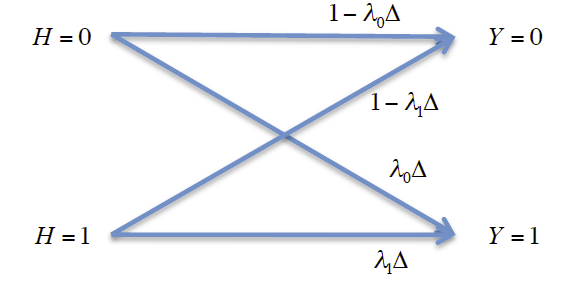
\includegraphics[width=8cm]{channel.png}
		\caption{Equivalent binary channel over time $\Delta$}
		\label{fig:channel}
	\end{figure}
	Since we obtained an approximation of a binary channel we may now ask how should $l(t)$ be decided in 
	other to maximize the mutual information of the binary channel
.\\\par	The Entropy can be calculated as follows
:\\	\begin{IEEEeqnarray*}{rCl}
		H(Y) 	& = & H_{b}[\Delta(\pi_{0}\lambda_{0} + \pi_{1}\lambda_{1})]
\\		H(Y|X) 	& = & \pi_{0}H_{b}(\Delta\lambda_{1}) + \pi_{1}H_{b}(\Delta\lambda_{1})
	\end{IEEEeqnarray*}
\\	Which gives us the mutual information of the channel
:\\	\begin{IEEEeqnarray*}{rCl}
		I(X;Y) 	& = & H(Y)-H(Y|X)
\\				& = & H_{b}[\Delta(\pi_{0}\lambda_{0} + \pi_{1}\lambda_{1})]
\\				&	& 	\> - \left[\pi_{0}H_{b}(\Delta\lambda_{1}) + \pi_{1}H_{b}(\Delta\lambda_{1})\right]
		\label{eq:dont_use_multline}
	\end{IEEEeqnarray*}
\\	Since we want to maximize the mutual information, we shall compare its derivative to zero
:\\	\begin{IEEEeqnarray*}{rCl}
		\frac{dI(X;Y)}{dl} 	& = & \log_{2}\left[\frac{1-\Delta[\pi_{0}\lambda_{0}+\pi_{1}\lambda_{1}]}{\Delta[\pi_{0}\lambda_{0}+\pi_{1}\lambda_{1}]}\right]2\Delta(\pi_{0}\sqrt{\lambda_{0}}+\pi_{1}\sqrt{\lambda_{1}})
\\							&	& 	\> - \log_{2}\left[\frac{1-\lambda_{0}\Delta}{\lambda_{0}\Delta}\right]2\Delta\pi_{0}\sqrt{\lambda_{0}}
\\							&	& 	\> - \log_{2}\left[\frac{1-\lambda_{1}\Delta}{\lambda_{1}\Delta}\right]2\Delta\pi_{1}\sqrt{\lambda_{1}}
\\							& = & 0
	\end{IEEEeqnarray*}
	\begin{IEEEeqnarray*}{rCl}
		\frac{dI(X;Y)}{dl} 	& = & \log_{2}\left[\frac{1-\Delta[\pi_{0}\lambda_{0}+\pi_{1}\lambda_{1}]}{\Delta[\pi_{0}\lambda_{0}+\pi_{1}\lambda_{1}]}\right]2\Delta(\pi_{0}\sqrt{\lambda_{0}}+\pi_{1}\sqrt{\lambda_{1}})
\\							&	& \> - 2\Delta\left[\log_{2}\left(\frac{1-\lambda_{0}\Delta}{\lambda_{0}\Delta}\right)\pi_{0}\sqrt{\lambda_{0}} + \log_{2}\left(\frac{1-\lambda_{1}\Delta}{\lambda_{1}\Delta}\right)\pi_{1}\sqrt{\lambda_{1}}\right]
\\							& = & 0
	\end{IEEEeqnarray*}
\\	In the optimal case where $l=l^{*}=\lStar$, we can calculate the following expressions for the $\lambda$'s
:\\	\begin{IEEEeqnarray*}{C}
		\lambda_{i} = (l^{*}+S_{i})^{2} = \left(\lStar+S_{i}\right)^{2} = \left(\frac{S_{0}\pi_{0} - S_{1}\pi_{1}+S_{i}(\pi_{1}-\pi_{0})}{\pi_{1}-\pi_{0}}\right)
	\end{IEEEeqnarray*}
\\	Which yields:
\\	\begin{IEEEeqnarray*}{r/C/l}
		\overline{\lambda} 	& = & \pi_{0}\lambda_{0}+\pi_{1}\lambda_{1}
\\							& = & \pi_{0}\left(\frac{\pi_{1}(S_{0}-S_{1})}{\pi_{1}-\pi_{0}}\right)^{2}
									+ \pi_{1}\left(\frac{\pi_{0}(S_{0}-S_{1})}{\pi_{1}-\pi_{0}}\right)^{2}
\\							& = & (\pi_{0}\pi_{1}^{2}+\pi_{1}\pi_{0}^{2})\left(\frac{(S_{0}-S_{1})}{\pi_{1}-\pi_{0}}\right)^{2}\IEEEyesnumber\label{eq:before_lambda_wave}
	\end{IEEEeqnarray*}\\
\\	Since $\pi_{0}+\pi_{1}=1$ we have that
:\\	\begin{IEEEeqnarray*}{r/C/l}
		\pi_{0}\pi_{1}^{2}+\pi_{1}\pi_{0}^{2} 	& = & \pi_{0}\pi_{1}(1-\pi_{0}) +\pi_{1}\pi_{0}^{2}				\\
												& = & \pi_{0}\pi_{1} - \pi_{0}\pi_{1}^{2} + \pi_{0}\pi_{1}^{2}	\\
												& = & \pi_{0}\pi_{1}
	\end{IEEEeqnarray*}
\\	Thus we can substitute in (\ref{eq:before_lambda_wave}) and get
:\\	\begin{IEEEeqnarray*}{r/C/l}
		(\pi_{0}\pi_{1}^{2}+\pi_{1}\pi_{0}^{2})\left(\frac{S_{0}-S_{1}}{\pi_{1}-\pi_{0}}\right)^{2} & = & \pi_{0}\pi_{1}\left(\frac{S_{0}-S_{1}}{\pi_{1}-\pi_{0}}\right)^{2}
	\end{IEEEeqnarray*}
\\	Overall we get the following expression for the $\lambda$'s:\\
\\	\curlyBracket{
		\lambda_{0} = \left(\frac{\pi_{1}(S_{0}-S_{1})}{\pi_{1}-\pi_{0}}\right)^{2}
\\		\lambda_{1} = \left(\frac{\pi_{0}(S_{0}-S_{1})}{\pi_{1}-\pi_{0}}\right)^{2}
\\		\overline{\lambda} = \pi_{0}\pi_{1}\left(\frac{S_{0}-S_{1}}{\pi_{1}-\pi_{0}}\right)^{2}
	}
\\	At this point we can derive the mutual information in the optimal case
:\\	\begin{IEEEeqnarray*}{r/C/l}
		I 	& = & H(Y) - H(Y|X)
\\			& = & \textcolor{BrickRed}{H_{b}[\lambdaWave\Delta]-\pi_{0}H_{b}(\lambda_{0}\Delta)-\pi_{1}H_{b}(\lambda_{1}\Delta)}
\\			& = & \textcolor{BrickRed}{\logH{\lambdaWave}-\pi_{0}\logH{\lambda_{0}}-\pi_{1}\logH{\lambda_{1}}}
\\			& = & \logH{\pi_{0}\pi_{1}\left(\frac{S_{0}-S_{1}}{\pi_{1}-\pi_{0}}\right)^{2}}
\\*			&	&		- \> \pi_{0}\logH{\left(\frac{\pi_{1}(S_{0}-S_{1})}{\pi_{1}-\pi_{0}}\right)^{2}}
\\*			&	&		- \> \pi_{1}\logH{\left(\frac{\pi_{0}(S_{0}-S_{1})}{\pi_{1}-\pi_{0}}\right)^{2}}
\\			& = & \pi_{0}\pi_{1}\left(\frac{S_{0}-S_{1}}{\pi_{1}-\pi_{0}}\right)^{2}
\\*			&	&		\left( 	- \log{\left[\pi_{0}\pi_{1}\left((\frac{(S_{0}-S_{1})}{\pi_{1}-\pi_{0}})\right)^{2}\right]}		\right.
\\*			&	&				+ \> \pi_{0}\log{\left[\left(\frac{\pi_{1}(S_{0}-S_{1})}{\pi_{1}-\pi_{0}})\right)^{2}\right]}
\\*			&	&		\left. 	+ \> \pi_{1}\log{\left[\left(\frac{\pi_{0}(S_{0}-S_{1})}{\pi_{1}-\pi_{0}})\right)^{2}\right]}	\right)
\\			& = & \pi_{0}\pi_{1}\left(\frac{S_{0}-S_{1}}{\pi_{1}-\pi_{0}}\right)^{2}
\\*			&	&		\left(	- \log{[\pi_{0}\pi_{1}]} - \cancel{\log{\left[\left((\frac{(S_{0}-S_{1})}{\pi_{1}-\pi_{0}})\right)^{2}\right]}}				\right.
\\*			&	&				+ \> 2\pi_{0}\log{[\pi_{0}]} + \cancel{\pi_{0}\log{\left[\left(\frac{(S_{0}-S_{1})}{\pi_{1}-\pi_{0}})\right)^{2}\right]}}
\\*			&	&		\left.	+ \> 2\pi_{1}\log{[\pi_{1}]} + \cancel{\pi_{1}\log{\left[\left(\frac{(S_{0}-S_{1})}{\pi_{1}-\pi_{0}})\right)^{2}\right]}} 	\right)
\\			& = & \pi_{0}\pi_{1}\left(\frac{S_{0}-S_{1}}{\pi_{1}-\pi_{0}}\right)^{2} ( - log{[\pi_{0}\pi_{1}]} + 2\pi_{0}\log{[\pi_{0}]} + \> 2\pi_{1}\log{[\pi_{1}]})
\\			& = & \pi_{0}\pi_{1}\left(\frac{S_{0}-S_{1}}{\pi_{1}-\pi_{0}}\right)^{2} ( - log{[\pi_{0}]} - log{[\pi_{1}]} + 2\pi_{0}\log{[\pi_{0}]} + \> 2\pi_{1}\log{[\pi_{1}]})
\\			& = & \pi_{0}\pi_{1}\left(\frac{S_{0}-S_{1}}{\pi_{1}-\pi_{0}}\right)^{2} ( (2\pi_{0}-1)log{[\pi_{0}]} + (2\pi_{1}-1)log{[\pi_{1}]}) \IEEEyesnumber\label{eq:before_two_pi}
	\end{IEEEeqnarray*}
\\	Again, since $\pi_{0}+\pi_{1}=1$ we have
:\\	\curlyBracket{
		2\pi_{0}-1=\pi_{0}+\pi_{0}-1=\pi_{0}-\pi_{1}
\\		2\pi_{1}-1=\pi_{1}+\pi_{1}-1=\pi_{1}-\pi_{0}
	}
\\	So we can substitute in (\ref{eq:before_two_pi}) and get
:\\	\begin{IEEEeqnarray*}{r/C/l}
		& = & \pi_{0}\pi_{1}\frac{(S_{0}-S_{1})^{2}}{(\pi_{1}-\pi_{0})^{\cancel{2}})} ( \cancel{(\pi_{0}-\pi_{1})}(log{[\pi_{0}]} - log{[\pi_{1}]}))
\\		& = & \> -\pi_{0}\pi_{1}\left(\frac{(S_{0}-S_{1})^{2}}{\pi_{1}-\pi_{0}}\right) log{\left[\frac{\pi_{0}}{\pi_{1}}\right]}
\\		& = & \pi_{0}\pi_{1}\left(\frac{(S_{0}-S_{1})^{2}}{\pi_{0}-\pi_{1}}\right) log{\left[\frac{\pi_{0}}{\pi_{1}}\right]}\IEEEyesnumber\label{eq:before_q}
	\end{IEEEeqnarray*}
\\	At this point we shall parameterize our probabilities with parameter $\g$ which will let us describe the recursive procedure in the system. That definition yields the parametrization
:\\	\curlyBracketFull{\g \Longrightarrow}{
		\pi_{0}=\piG{0}
\\		\pi_{1}=\piG{1}
	}
\\	With that parameterization, we can now continue developing (\ref{eq:before_q})
:\\	\begin{IEEEeqnarray*}{r/C/l}
		\pi_{0}\pi_{1}\left(\frac{(S_{0}-S_{1})^{2}}{\pi_{0}-\pi_{1}}\right) log{\left[\frac{\pi_{0}}{\pi_{1}}\right]}
			& = & (\piG{0})(\piG{1})\frac{(S_{0}-S_{1})^{2}}{\piG{0}-\piG{1}}log{\left(\frac{\piG{0}}{\piG{1}}\right)}
\\			& = & \left(\frac{g}{(1+g)^{\cancel{2}}}\right)\left(\frac{(S_{0}-S_{1})^{2}}{\frac{g-1}{\cancel{1+g}}}\right)\log{(g)}
\\			& = & \frac{g(S_{0}-S_{1})^{2}}{(1-g)(1+g)}\log{(g)}
	\end{IEEEeqnarray*}
\\	We can also recompute the entropy using that parameterization
:\\	\begin{IEEEeqnarray*}{r/C/l}
		H(g) 	& = & H_{b}(\pi_{0},\pi_{1})
\\				& = & \logH{\pi_{0}}+\logH{\pi_{1}}
\\				& = & \logH{\piG{0}}+\logH{\piG{1}}
\\				& = & \> - \piG{1}\left(g\log{\piG{0}}+\log{\piG{1}}\right)
\\				& = & \> - \piG{1}\left(g\log{g}+(1+g)\log{\piG{1}}\right)
\\				& = & \> \piG{1}\left(\logHminus{(1+g)}-\logHminus{g}\right)
\\				& = & \> \log{(1+g)}-\piG{0}\log{g}
	\end{IEEEeqnarray*}
\\	So we can now find the derivative of the entropy as a function of $g$
:\\	\begin{IEEEeqnarray*}{r/C/l}
		\frac{H(g)}{dg} & = & \frac{d(\log{(1+g)}-\piG{0}\log{g})}{dg}
\\						& = & \piG{1}-\frac{(1+\cancel{g})-\cancel{g}}{(1+g)^{2}}\log{g}-\frac{1}{\cancel{g}}\frac{\cancel{g}}{\left(1+g\right)}
\\						& = & \cancel{\piG{1}}-\frac{\log{g}}{(1+g)^{2}}-\cancel{\piG{1}}
\\						& = & \> - \frac{\log{g}}{(1+g)^{2}}
	\end{IEEEeqnarray*}
\\	Each step of the recursion, the entropy is lowered since we have more certainty of our choice. The quantity of the change in certainty can be describe by the following equation
:\\	\begin{IEEEeqnarray*}{r/C/l}
		H(g(t+\Delta)) & = & H(g(t))-\Delta I(g(t))
	\end{IEEEeqnarray*}
\\	If we look again at the the derivative of the entropy, we see than indeed it is negative which coincides with the fact that the certainty is increasing
.\\\par	The definition of the derivative entropy by $g$, is defined by
:\\	\begin{IEEEeqnarray*}{r/C/l}
		\frac{H(g)}{dg} & = & \frac{H(g(t+\Delta))-H(g(t))}{g(t+\Delta)-g(t)}
	\end{IEEEeqnarray*}
\\	which yields
:\\	\begin{IEEEeqnarray*}{r?r/C/l}
		\Longrightarrow & g(t+\Delta) & = & g(t)+\frac{- \Delta I}{\frac{dH}{dg}} \IEEEyesnumber\label{eq:g_change}
	\end{IEEEeqnarray*}
\\	Since we found already the derivative and the mutual information, we can substitute them in (\ref{eq:g_change})
:\\	\begin{IEEEeqnarray*}{r/C/l}
		g(t+\Delta) & = & g(t)+\frac{- \Delta I}{\frac{dH}{dg}}
\\					& = & g(t)+\frac{- \Delta\frac{g(S_{0}-S_{1})^{2}}{(1-g)\cancel{(1+g)}}\cancel{\log{(g)}}}{-\frac{\cancel{\log{(g)}}}{(1+g)^{\cancel{2}}}}
\\					& = & g(t)+\left(\frac{\Delta g(1+g)}{(1-g)}\right)(S_{0}-S_{1})^{2}
	\end{IEEEeqnarray*}

% 	:\\	\begin{IEEEeqnarray*}{r/C/l}
% 		g(t+\Delta) & = & g(t)+\frac{- \Delta I}{\frac{dH}{dg}}
% \\					& = & g(t)+\frac{- \Delta\frac{g(S_{0}-S_{1})^{2}}{(1-g)\cancel{(1+g)}}\cancel{\log{(g)}}}{-\frac{\cancel{\log{(g)}}}{(1+g)^{\cancel{2}}}}
% \\					& = & g(t)+\left(\frac{\Delta g(1+g)}{(1-g)}\right)(S_{0}-S_{1})^{2}
% 	\end{IEEEeqnarray*}
\end{document}


% *** Notes *** %

% \begin{Notes}
	% Cool macro: \newcommand{\divbytwo}[1]{\frac{#1}{2}}
	
	% \quad - tab
	% \qquad = big tab
	
	% \usepackage{xparse}
	% \NewDocumentCommand\TwoArgs{mm}{Text using #1 and #2}
	% \NewDocumentCommand\OneOptOfTwo{O{}mm}%
	% {Text with #2, #3 and perhaps #1}
	% \NewDocumentCommand\OneOptOfTwoWithTest{om}{%
	% 	\IfNoValueTF{#1}
	% 	{Do stuff with #2 only}
	% 	{Do stuff with #1 and #2}%
	% }
	% \NewDocumentCommand\StarThenArg{sm}{%
	% 	\IfBooleanTF#1
	% 	{Use #2 with a star}
	% 	{Use #2 without a star}%
	% }

	% Change margin:
	% \begin{changemargin}{-1cm}{-1cm} 
	% \end{changemargin}

	% Brackets:

	% Sizes of brackets:
	% \bigl, \Bigl, \biggl, and \Biggl
	
	% \begin{equation*}
	% 	\left\| \left(
	% 	\left[ \left\{ \left|
	% 	\left\lfloor \left\lceil
	% 	\frac{1}{2}
	% 	\right\rceil \right\rfloor
	% 	\right| \right\} \right]
	% 	\right) \right\|
	% \end{equation*}

	% \begin{IEEEeqnarray}{rCl}
	% 	a & = & \log \left( 1 \right.
	% 	\nonumber\\
	% 	&& \qquad \left. + \>
	% 	\frac{b}{2} \right)
	% 	\label{eq:wrong_try}
	% \end{IEEEeqnarray}

	% \begin{IEEEeqnarray}{rCl}
	% 	a & = & \log \Biggl( 1
	% 	\nonumber\\
	% 	&& \qquad +\>
	% 	\frac{b}{2} \biggr)
	% \end{IEEEeqnarray}

	% IEEE

		% \> manually unary to binary
		% {} manually binary to unary

		% Spaces:
		% added by . and / and ? and " in increasing order.

		% hyperlinks:

		% We have
		% \begin{IEEEeqnarray}{rCl}
		% 	\subnumberinglabel{eq:block2}
		% 	a & = & b + c
		% 	\label{eq:block2_eq1}\\
		% 	& = & d + e
		% 	\label{eq:block2_eq2}
		% \end{IEEEeqnarray}
		% and
		% \begin{IEEEeqnarray}{c}
		% 	\IEEEyessubnumber*
		% 	f = g - h + i
		% 	\label{eq:block2_eq3}
		% \end{IEEEeqnarray}
	
		% lala (\ref{eq:block2_eq3}) haha\\

	% Frame:

	% \begin{equation*}
	% 	\newlength{\fboxstore}
	% 	\setlength{\fboxstore}{\fboxsep}
	% 	\setlength{\fboxsep}{6pt}
	% 	\boxed{
	% 		= \left\{ \,
	% 		\begin{IEEEeqnarraybox}[][c]{l"s}
	% 			\IEEEstrut
	% 				\lambda_{0} = \left(\frac{\pi_{1}(S_{0}-S_{1})}{\pi_{1}-\pi_{0}}\right)^{2}							\\
	% 				\lambda_{1} = \left(\frac{\pi_{0}(S_{0}-S_{1})}{\pi_{1}-\pi_{0}}\right)^{2}							\\
	% 				\overline{\lambda} = \pi_{0}\pi_{1}\left(\frac{S_{0}-S_{1}}{\pi_{1}-\pi_{0}}\right)^{2}
	% 			\IEEEstrut
	% 		\end{IEEEeqnarraybox}
	% 		\right.
	% 	}
	% 	\setlength{\fboxsep}{\fboxstore}
	% \end{equation*}

% \end{Notes}

% ************* %